%%%%%%%%%%%%%%%%%%%%%%%%%%%%%%%%%%%%%%%%%%%%%%%%%%%%%%%%
%%%%%%%%%%%%%%%%%%%%%%%%%%%%%%%%%%%%%%%%%%%%%%%%%%%%%%%%
\section[Analysis]{Search for a single produced \Tp~decaying into top and Higgs in the full hadronic final state}
\setcounter{tocdepth}{2}

\begin{frame}
\begin{center}
Search for a single produced \Tp~decaying into top and Higgs in the full hadronic final state
\end{center}
\end{frame}


\subsection{Introduction - Analysis Strategy}
\begin{frame}{Introduction - Analysis Strategy}
\vspace{-.2cm}
\begin{columns}

\begin{column}{.50\textwidth}
\begin{block}{}
\begin{itemize}\scriptsize
\item Single produced \Tp~with an associated jet
\item Full hadronic final state: \\ $T'\to t H \to b W^{+} \bar{b} b \to b \bar{b} j j b$
\item Reconstruction of \Tp~mass: $M(5j)$
\item Main challenges:
  \begin{itemize}\scriptsize
  \item Huge backgrounds $\rightarrow$ Mainly QCD and \ttbar
  \item \Tp~reconstruction with high jet multiplicity
  \end{itemize}
\item Fundamental tools for background discrimination:
  \begin{itemize}\scriptsize
  \item B-tagged jets multiplicity
  \item \Tp~reconstruction procedure
  \end{itemize}
\end{itemize}
\end{block}
\end{column}

\begin{column}{.50\textwidth}
\begin{center}
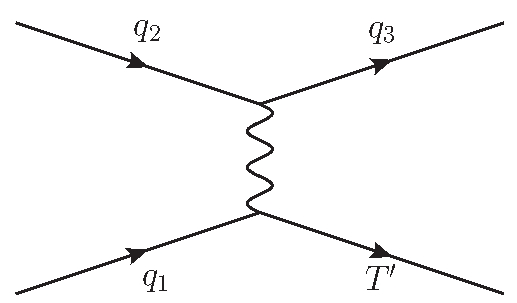
\includegraphics[width=0.9\textwidth]{../figs/Tchannel_T_single.jpg}\\
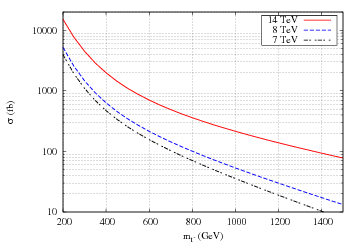
\includegraphics[width=1.0\textwidth]{../figs/pheno_prod_single_tp.png}
\end{center}
\end{column}
\end{columns}

\end{frame}

\begin{frame}{Datasets}
\vspace{-.2cm}

%\begin{table*}[htbH]
\begin{center}
\resizebox{\textwidth}{!}{
\begin{tabular}{|c|c|}
\hline 
Dataset name & Int. Luminosity ($\text{pb}^{-1}$) \\
\hline
/MultiJet/Run2012A-22Jan2013-v1/AOD & 889.4 \\
/MultiJet1Parked/Run2012B-05Nov2012-v2/AOD & 4429.0 \\
/MultiJet1Parked/Run2012C-part1-05Nov2012-v2/AOD & 494.6 \\
/MultiJet1Parked/Run2012C-part2-05Nov2012-v2/AOD & 6654.0 \\
/MultiJet1Parked/Run2012D-part1-10Dec2012-v1/AOD & 5955.1 \\
/MultiJet1Parked/Run2012D-part2-17Jan2013-v1/AOD & 734.0 \\
/MultiJet1Parked/Run2012D-part2-PixelRecover-17Jan2013-v1 & 538.4 \\
\hline
\multicolumn{1}{|r|}{\textit{Total}} & 19694.5 \\
\hline
\end{tabular}
}
%\caption{List of Multijet Primary Dataset used in the analysis and the corresponding integrated luminosity calculated using the golden JSON (Java Script Object Notation) file. The golden JSON file contains the information about the luminosity sections considered as good for all runs. A good luminosity section is defined as a luminosity section where the detector was fully functioning, this is all subsystems were taking data and without problems.  \label{tab:datasets}}
\end{center}
%\end{table*}

%\begin{table*}[htbH]
\begin{center}
\resizebox{\textwidth}{!}{
\begin{tabular}{|c|c|c|}
\hline 
Samples & Cross-Section (pb) & Number of events\\
\hline
QCD\_Pt-120to170\_TuneZ2star\_8TeV\_pythia6 & 16\(\times 10^4\) & 5.9M\\
QCD\_Pt-170to300\_TuneZ2star\_8TeV\_pythia6 & 34\(\times 10^3\) & 5.8M\\
QCD\_Pt-300to470\_TuneZ2star\_8TeV\_pythia6 & 18\(\times 10^2\) & 5.9M\\ 
QCD\_Pt-470to600\_TuneZ2star\_8TeV\_pythia6 & 114 & 3.9M\\
QCD\_Pt-600to800\_TuneZ2star\_8TeV\_pythia6 & 27 & 3.9M\\
QCD\_Pt-800to1000\_TuneZ2star\_8TeV\_pythia6 & 3.5 & 3.9M\\
QCD\_HT-500To1000\_TuneZ2star\_8TeV-madgraph-pythia6 & 84\(\times 10^2\) & 30M\\ 
QCD\_HT-1000ToInf\_TuneZ2star\_8TeV-madgraph-pythia6 & 2\(\times 10^2\) & 14M\\ 
TTJets\_MSDecays\_central\_TuneZ2star\_8TeV-madgraph-tauola & 247.7 [NNLO] & 62M\\
TprimeJetToTH\_\textbf{M-700}\_TuneZ2star\_8TeV-madgraph\_tauola & 143.7 & 99K \\
\hline
\end{tabular}
}
%\caption{List of Monte-Carlo background samples used in the analysis, their corresponding cross-section and their number of events.\label{tab:MCbkg}}
\end{center}
%\end{table*}

\tiny{Signal samples were done with $T'\to tH$ with $H\to\tau^{+}\tau^{-}$ (6\%) and $H\to b\bar{b}$ (94\%). Correction with weight of 0.61 to obtain correct $Br(H\to b\bar{b})=0.57$. }

\end{frame}